
\documentclass{beamer} 


\mode<presentation>
{
  \usetheme{Berkeley}
  % or ...

  \setbeamercovered{transparent}
  % or whatever (possibly just delete it)
}

\usepackage{tikz}
\usepackage{graphicx}
\usepackage[english]{babel}


\usepackage[utf8]{inputenc}
% or whatever

\usepackage{times}
\usepackage[T1]{fontenc}
% Or whatever. Note that the encoding and the font should match. If T1
% does not look nice, try deleting the line with the fontenc.


\title[Reproducible Coding Strategies] % (optional, use only with long paper titles)
{Reproducible Coding Strategies}

\subtitle
{}

\author[Christensen] % (optional, use only with lots of authors)
{Garret~Christensen\inst{1}}
% - Give the names in the same order as the appear in the paper.
% - Use the \inst{?} command only if the authors have different
%   affiliation.

\institute[Universities of Somewhere and Elsewhere] % (optional, but mostly needed)
{
  \inst{1}%
  UC Berkeley:\\
  Berkeley Initiative for Transparency in the Social Sciences\\
  Berkeley Institute for Data Science\\
  }
% - Use the \inst command only if there are several affiliations.
% - Keep it simple, no one is interested in your street address.

\date[BITSS2014] % (optional, should be abbreviation of conference name)
{IDB, March 2018\\
Slides available online at \url{http://www.github.com/BITSS/IDBMarch2018}}
% - Either use conference name or its abbreviation.
% - Not really informative to the audience, more for people (including
%   yourself) who are reading the slides online

\subject{Research Transparency}
% This is only inserted into the PDF information catalog. Can be left
% out. 

\pgfdeclareimage[height=2cm]{university-logo}{../Images/BITSSlogo.png}
\logo{\pgfuseimage{university-logo}}

% If you have a file called "university-logo-filename.xxx", where xxx
% is a graphic format that can be processed by latex or pdflatex,
% resp., then you can add a logo as follows:

% \pgfdeclareimage[height=0.5cm]{university-logo}{university-logo-filename}
% \logo{\pgfuseimage{university-logo}}



% Delete this, if you do not want the table of contents to pop up at
% the beginning of each subsection:
%\AtBeginSubsection[]
%{
%  \begin{frame}<beamer>{Outline}
%    \tableofcontents[currentsection,currentsubsection]
%  \end{frame}
%}


% If you wish to uncover everything in a step-wise fashion, uncomment
% the following command: 

\beamerdefaultoverlayspecification{<.->}


\begin{document}

\begin{frame}
  \titlepage
\end{frame}




% Structuring a talk is a difficult task and the following structure
% may not be suitable. Here are some rules that apply for this
% solution: 

% - Exactly two or three sections (other than the summary).
% - At *most* three subsections per section.
% - Talk about 30s to 2min per frame. So there should be between about
%   15 and 30 frames, all told.

% - A conference audience is likely to know very little of what you
%   are going to talk about. So *simplify*!
% - In a 20min talk, getting the main ideas across is hard
%   enough. Leave out details, even if it means being less precise than
%   you think necessary.
% - If you omit details that are vital to the proof/implementation,
%   just say so once. Everybody will be happy with that.
%%%%%%%%%%%%%%%%%%%%%%%%%%%%%%%%%%%%%%%%%%%%%%%%%%%%%%%%%%%%%%%%%%%%%%%
%%%%%%%%%%%%%%%%%%%%%%%%%%%%%%%%%%%%%%%%%%%%%%%%%%%%%%%%%%%%%%%%%%%%%
\begin{frame}{Outline}
  \tableofcontents
  % You might wish to add the option [pausesections]
\end{frame}

\section {Principles}
{ % all template changes are local to this group.
    \setbeamertemplate{navigation symbols}{}
    \begin{frame}[plain]
        \begin{tikzpicture}[remember picture,overlay]
            \node[at=(current page.center)] {
                \href{https://www.bitss.org/}{\includegraphics[width=\paperwidth]{../Images/bitsslogo.png}}
            };
        \end{tikzpicture}
     \end{frame}
}

\begin{frame}{The Claerbout Principle}

\begin{quote}``An article about computational science in a scientific publication is not the scholarship itself, it is merely advertising of the scholarship. The actual scholarship is the complete software development environment and the complete set of instructions which generated the figures.'' 

\href{https://statweb.stanford.edu/~wavelab/Wavelab_850/wavelab.pdf}{(Buckheit \& Donoho, 1995)}\end{quote}
\end{frame}

\begin{frame}{Organizing Principles}
\begin{enumerate}
	\item Use code (scripts), don't work by hand (Excel/spreadsheet, GUIs).
	\item Consider not saving statistical output, and just saving the code and raw data that generates it.
	\item Reproducibility--on your own machine across multiple runs, across machines, across researchers. 
\end{enumerate}
\end{frame}

\begin{frame}{File Management \& Coding Suggestions}
Begin with a logical file structure 
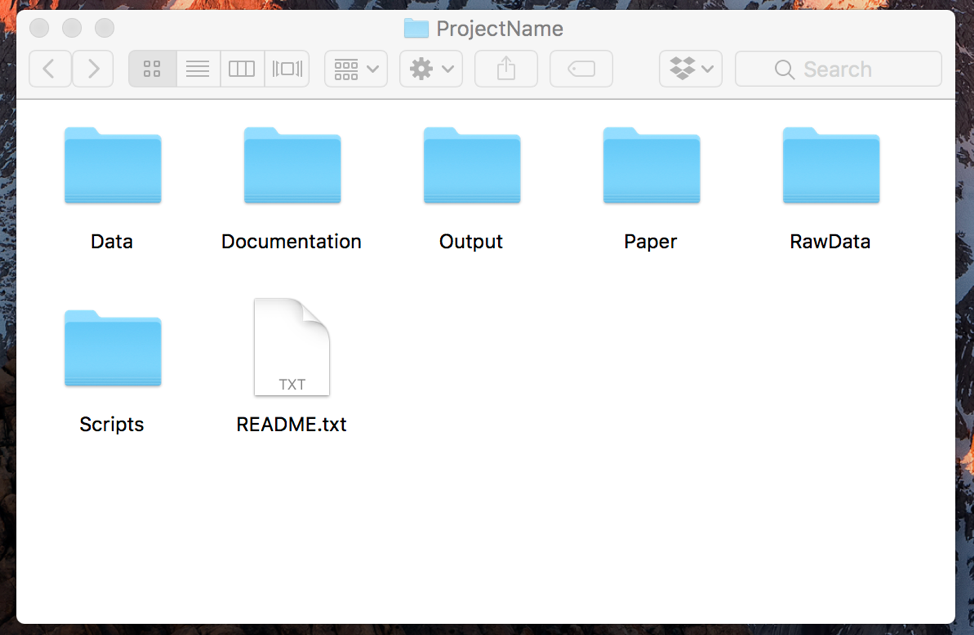
\includegraphics[height=2.25in]{../Images/files.png}
\end{frame}


\section{General Coding Suggestions}
\begin{frame}{General Coding Suggestions}

\begin{itemize} 
\item Make sure script files are self-contained: don't write code that only works if you run a group of other files previously in a specific order and then leave things hanging precariously. 

\item Include tests in your code.   
This can alert you if output changes. 

\item You can never comment your code too much. Truly explain rather than transliterating: \texttt{x=1} as "initialize the population count to 1" or "set x equal to 1."
 
\item Indent your code.   
\end{itemize}
\end{frame}

\begin{frame}{General Coding Suggestions II}
\begin{itemize}
\item  Once posted, any changes at all require a new file name. Better: use version control.  

\item  Separate your data cleaning and analysis files. Don't make any new variables that need saving (or will be used by multiple analysis files) in an analysis file. It is far better to only create a variable once so you know that it is identical when used in different analysis files.
\end{itemize}
\end{frame}


\begin{frame}{General Coding Suggestions III}
\begin{itemize}

\item  Name variables informatively: pick a side for indicator variables ``dead" (or ``living'') instead of ``status". (gender, race, etc.)

\item Don't leave clutter around-delete temporary or unnecessary intermediate objects. 

\item You can use a prefix such as \texttt{x\_} or \texttt{temp\_} so you know which files or variables can easily be deleted later. Stata also has the \texttt{tempfile} and \texttt{tempvar} functionality.  

\item Every variable should have a label. (If allowed for by the program.)

\item  Use relative directory paths (such as ``./Data" not ``C:/Users/garret/Documents/Project/Data") 

\end{itemize}
\end{frame}


\section{Stata Suggestions}
\begin{frame}{Stata Suggestions}
\begin{itemize}
\item Accurately and concisely capture missing values. (`.` and `.a-.z`)

\item Make sure code always produces the same result, and that merging and sorting is reproducible. `duplicates report; isid; sort, stable`  

\item	Run tests to alert yourself when results change. 
\end{itemize}
\end{frame}

\begin{frame}{Example Test}
\texttt{count if \_merge!=3 \\ if r(N)!=74 \{ \\ display "Unmatched observations changed!" \\ there is an error here \\  \}   }
\end{frame}
   
\begin{frame}
 \begin{itemize}
\item	Don't use abbreviations for variables, or commands beyond reason
\item	Use global macros to define directory paths so collaborators can readily work across different computers.
\item	Use local macros for varlists.
\end{itemize}
\end{frame}


\begin{frame}{Stata Suggestions}
\begin{itemize}
\item Use computer-stored versions of numerical output (eg `r(mean)`). Use `return list` and `ereturn list`
\item	If you have a master .do file that calls other .do files, which each have their own .log file capturing output, you can run multiple log files at the same time (so you end up with a master .log file)
\item	Use the `label data` and `notes`.
\item	Use the `notes` command for variables as well for identifying information that is too long for the variable label.
\end{itemize}
\end{frame}


\begin{frame}{Stata Suggestions}
\begin{itemize}
\item	Validate data sources to ensure consistency. Use `datasignature` on auto data set (`sysuse auto.dta`, then `datasignature set` should give you this number: `74:12(71728):3831085005:1395876116`) 
\item	Use value labels for all categorical variables. `numlabel [lblname-list], add command.`  
\item	Don't use capital letters in variable names.
\item	Make your files as non-proprietary as possible (use the `saveold` command) 

\end{itemize}
\end{frame}

%%%%%%%%%%%%%%%%%%%%%%%%%%%%%%%%%%%%%%%%%%%%%%%%%%%%%%%%%%%%%%%%%%%%%%%%%%

\begin{frame}
\begin{center}
Questions?
\vspace{1in}


\Huge{Thank you!}
\end{center}
\end{frame}

\end{document}

